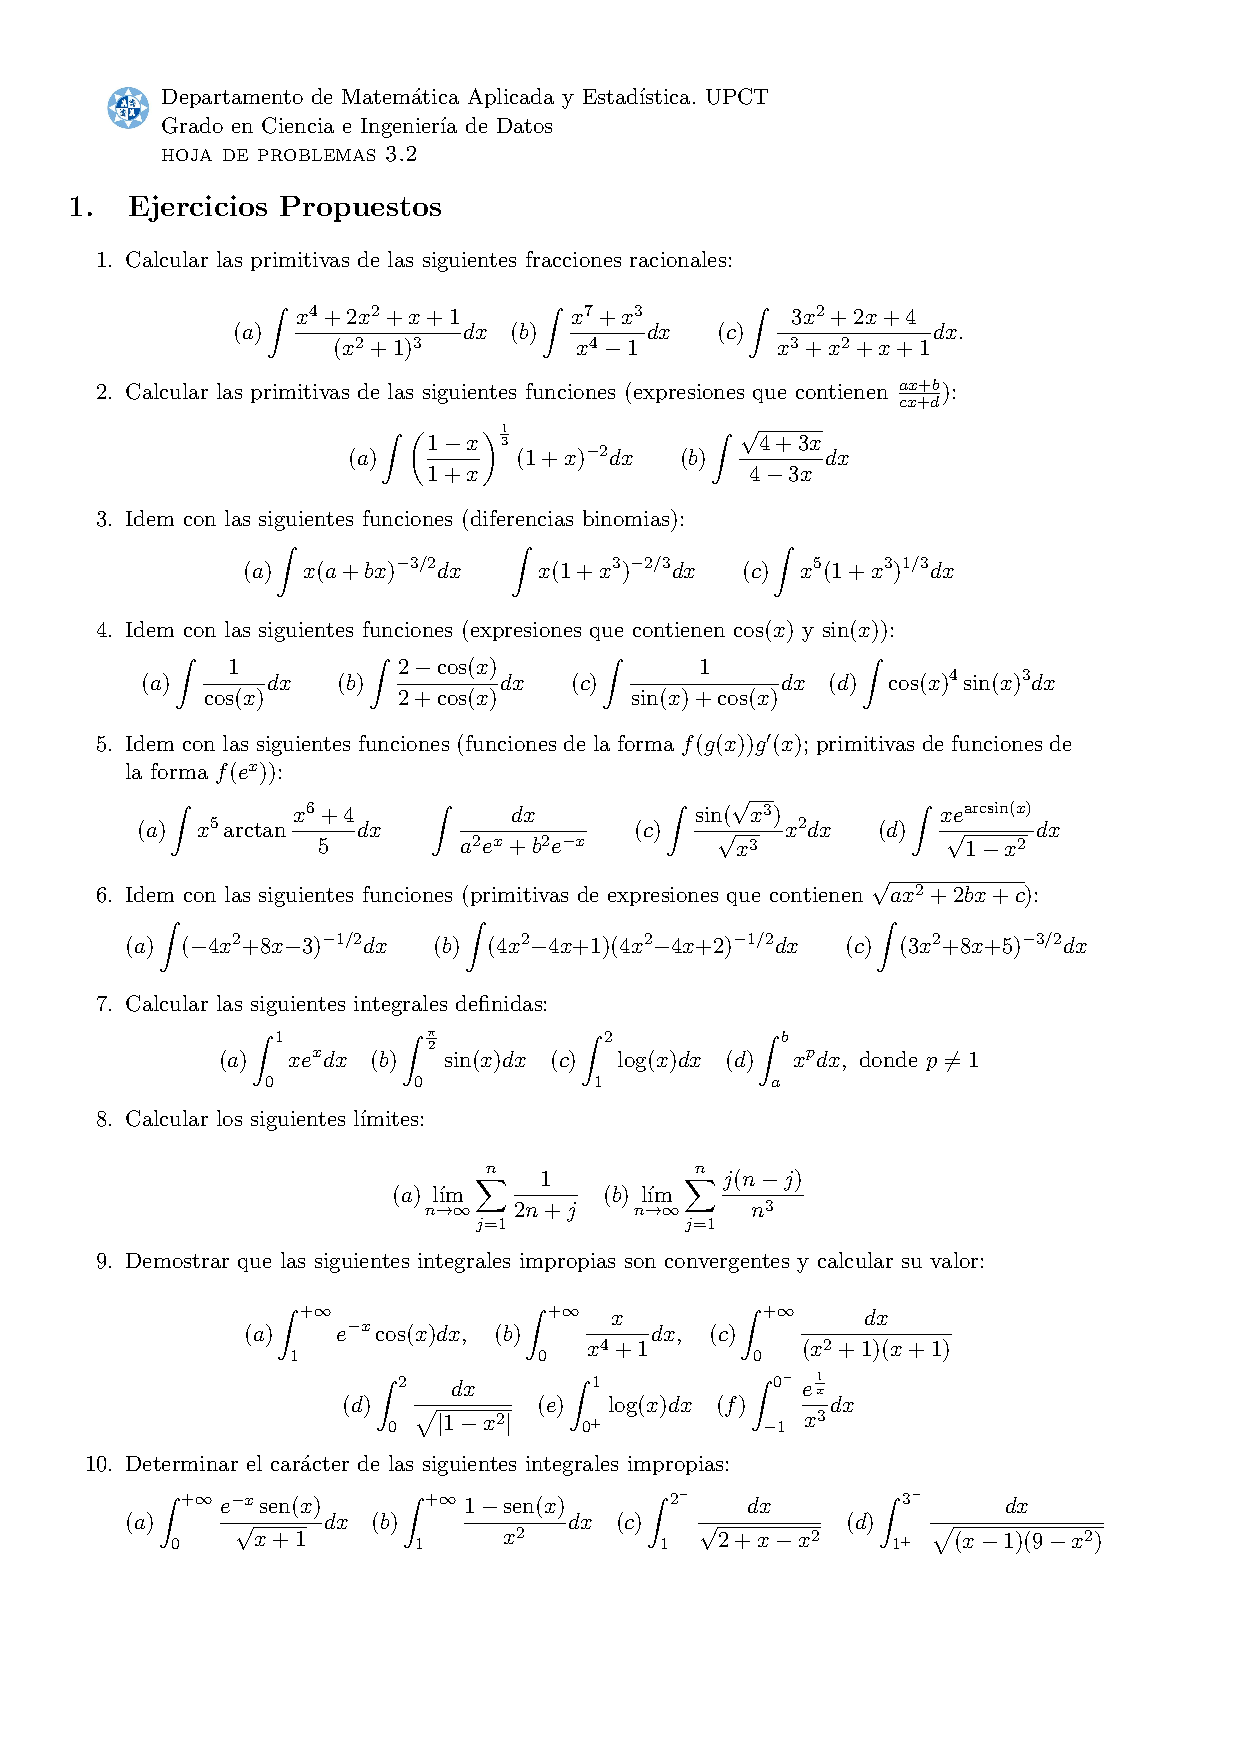
\includepdf[pages=-]{Tareas/Tema 3/Hoja 3.2/Hoja 3.2.pdf}

\begin{enumerate}[label=\color{red}\textbf{\arabic*)}, leftmargin=*]
	\item \lb{Calcular las primitivas de las siguientes fracciones racionales:}
	\begin{enumerate}[label=\color{red}\alph*)]
		\item $\db{\int\dfrac{x^4+2x^2+x+1}{(x^2-1)^3}\dx=}\int\dfrac{}{}$
		\item $\db{\int\dfrac{x^7+x^3}{x^4-1}\dx=}\int\dfrac{x^3(x^4+1)}{(x^2+1)(x+1)(x-1)}=$
		\item $\db{\int\dfrac{3x^2+2x+4}{x^3+x^2+x+1}\dx=}\int\dfrac{}{(x+1)(x^2+1)}$
            
            
	\end{enumerate}
	\item \lb{Calcular las primitivas de las siguientes funciones $\left(\text{expresiones que contienen  }\dfrac{ax+b}{cx+d}\right)$:}
	\begin{enumerate}[label=\color{red}\alph*)]
		\item $\db{\int\left(\dfrac{1-x}{1+x}\right)^{\frac{1}{3}}(1+x)^{-2}\dx}$
            
            $\begin{array}{l}
                  \begin{array}{l}
                  \begin{aligned}
                        \dfrac{1-x}{1+x}=t^3\longrightarrow&1-x=t^3\cdot(1+x)\\
                        &1-x=t^3+t^3x\\
                        &1-t^3=x(1+t^3)\\
                  \end{aligned}\\
                  x=\dfrac{1-t^3}{1+t^3} \\
                        \dx=\dfrac{-3t^2\cdot(1+t^3)-(1-t^3)\cdot3t^2}{(1+t^3)^2}\dt=\dfrac{-t^2-\cancel{3t^5}-3t^2+\cancel{3t^5}}{(1+t^3)^2}\dt=\dfrac{-6t^2}{(1+t^3)^2}\dt
            \end{array}\\
            \begin{aligned}
                  \int(t^3)^{\frac{1}{3}}\cdot\left(1+\dfrac{1-t^3}{1+t^3}\right)^{-2}\cdot\dfrac{-6t^2}{(1+t^3)^2}\dt&=\int t\cdot\left(\dfrac{2}{1+t^3}\right)^{-2}\cdot\left(\dfrac{-6t^2}{(1+t^3)^2}\right)\dt=\int-\dfrac{6}{4}\cdot t^3\dt\\
                  &=\bboxed{-\dfrac{3}{2}\cdot\dfrac{t^4}{4}+\mathrm{C}}
            \end{aligned}
            \end{array}$
		\item $\db{\int\dfrac{\sqrt{4+3x}}{4-3x}\dx}$
	\end{enumerate}
	\item \lb{Ídem con las siguientes funciones (diferencias binomias):}
	\begin{enumerate}[label=\color{red}\alph*)]
		\item $\db{\int x(a+bx)^{-\frac{3}{2}}\dx}$
		\item $\db{\int x(1+x^3)^{-\frac{2}{3}}\dx}$
		\item $\db{\int x^5(1+x^3)^{\frac{1}{3}}\dx}$
	\end{enumerate}
	\item \lb{Ídem con las siguientes funciones (expresiones que contienen $\cos(x)$ y $\sin(x)$):}
	\begin{enumerate}[label=\color{red}\alph*)]
		\item $\db{\int\dfrac{1}{\cos(x)}\dx=}\int\dfrac{\cancel{1+t^2}}{1-t^2}\cdot\dfrac{2\dt}{\cancel{1+t^2}}=\int\dfrac{2\dt}{1-t^2}=2\int\dfrac{\dt}{(1-t)(1+t)}=\int\dfrac{A}{1-t}+\dfrac{B}{1+t}\dt$
            
            $\begin{array}{l|l|ll}
                  t=\tan(x) & f\left(\cos(x)\right)=\dfrac{1}{\cos(x)} & t=\sin(x) & \dt=\cos(x)\dx\\
                  \cos(x)=\dfrac{1-t^2}{1+t^2} & f\left(-\cos(x)\right)=\dfrac{1}{-\cos(x)}=-f\left(\cos(x)\right) & \cos(x)=\sqrt{1-t^2} & \dx=\dfrac{\dt}{\sqrt{1-t^2}}\\
                  \dx=\dfrac{2\dt}{1+t^2} & & &
            \end{array}$
		\item $\db{\int\dfrac{2-\cos(x)}{2+\cos(x)}\dx}$
		\item $\db{\int\dfrac{1}{\sin(x)+\cos(x)}\dx}$
		\item $\db{\int\cos(x)^4\sin(x)^3\dx}$
	\end{enumerate}
	\item \lb{Ídem con las siguientes funciones (funciones de la forma $f\left(g(x)\right)g'(x)$; primitivas de funciones de la forma $f(e^x)$):}
	\begin{enumerate}[label=\color{red}\alph*)]
		\item $\db{\int x^5\arctan\dfrac{x^6+4}{5}\dx}$
		\item $\db{\int\dfrac{\dx}{a^2e^x+b^2e^{-x}}}$
		\item $\db{\int\dfrac{\sin(\sqrt{x^3})}{\sqrt{x^3}}x^2\dx}$
		\item $\db{\int\dfrac{xe^{\arcsin(x)}}{\sqrt{1-x^2}}\dx}$
	\end{enumerate}
	\item \lb{Ídem con las siguientes funciones (primitivas de expresiones que contienen $\sqrt{ax^2+2bx+c}$):}
	\begin{enumerate}[label=\color{red}\alph*)]
		\item $\db{\int(-4x^2+8x-3)^{-\frac{1}{2}}\dx}$
		\item $\db{\int(4x^2-4x+1)(4x^2-4x+2)^{-\frac{1}{2}}\dx}$
		\item $\db{\int(3x^2+8x+5)^{-\frac{3}{2}}\dx}$
	\end{enumerate}
	\item \lb{Calcular las siguientes integrales definidas:}
	\begin{enumerate}[label=\color{red}\alph*)]
		\item $\db{\int_{0}^{1}xe^x\dx}$
		\item $\db{\int_{0}^{\frac{\pi}{2}}\sin(x)\dx}$
		\item $\db{\int_{1}^{2}\log(x)\dx}$
		\item $\db{\int_{a}^{b}x^p\dx,\:\text{donde }p\neq1}$
	\end{enumerate}
	\item \lb{Calcular los siguientes límites:}
	\begin{enumerate}[label=\color{lightblue}\arabic*)]
		\item $\db{\lim_{n\to\infty}\sum_{j=1}^{n}\dfrac{1}{2n+j}=}\lim_{n\to\infty}\sum_{j=1}^{n}\dfrac{1}{n\cdot\left(2+\frac{j}{n}\right)}=\lim_{n\to\infty}\sum_{j=1}^{n}\dfrac{1}{n}\cdot f\left(\dfrac{j}{n}\right)=\int_{0}^{1}f(x)\dx=\int_{0}^{1}\dfrac{1}{2+x}\dx=\left[\log(x^2)\right]_{0}^{1}=\log(3)-\log(2)=\log\left(\dfrac{3}{2}\right)$
            
            
		\item $\db{\lim_{n\to\infty}\sum_{j=1}^{n}\dfrac{j(n-j)}{n^3}=}$
	\end{enumerate}
	\item \lb{Demostrar que las siguientes integrales impropias son convergentes y calcular su valor:}
	\begin{enumerate}[label=\color{red}\alph*)]
		\item $\db{\int_{1}^{+\infty}e^{-x}\cos(x)\dx=}\lim_{n\to\infty}\dfrac{\tozero{e^{-x}}\sin(x)-\tozero{e^{-x}}\cos(x)}{2}-\left(\dfrac{e^{-1}\sin(1)-\cos}{}\right)$
            
            $\begin{array}{l|l}
                  \multicolumn{2}{l}{\int e^{-x}\cos(x)\dx=e^{-x}\sin(x)+\int e^{-x}\sin(x)\dx=e^{-x}\sin(x)-e^{-x}\cos(x)-\int e^{-x}\cos(x)\dx}\\
                  \begin{array}{ll}
                        u=e^{-x} & \du=-e^{-x}\dx\\
                        \dv=\cos(x)\dx & v=\sin(x)
                  \end{array} & \begin{array}{l}
                  u=e^{-x}
                  \end{array}
            \end{array}$
		\item $\db{\int_{0}^{+\infty}\dfrac{x}{x^4+1}\dx=}\int_{0}^{1}\dfrac{x}{x^4+1}\dx+\int_{1}^{+\infty}\dfrac{x}{x^4+1}\dx=\lim_{n\to\infty}\arctan(x^2)-\arctan(0)=\dfrac{\pi}{2}-0=\bboxed{\dfrac{\pi}{2}}$
            
            $\begin{array}{l|l}
                  \begin{array}{l}
                        \lim_{n\to\infty}\dfrac{\frac{x}{x^4+1}}{\frac{1}{x^3}}=1\\
                        \int_{1}^{+\infty}\dfrac{1}{x^3}\dx\text{ es convergente }
                  \end{array} & \int\dfrac{x}{x^4+1}\dx=\dfrac{1}{2}\int\dfrac{2x}{(x^2)^2+1}\dx=\dfrac{1}{2}\arctan(x^2)+\mathrm{C}
            \end{array}$
		\item $\db{\int_{0}^{+\infty}\dfrac{\dx}{(x^2+1)(x+1)}}$
            
            $\dfrac{1}{(x^2+1)(x+1)}=\dfrac{A}{x+1}+\dfrac{Mx+N}{x^2+1}=\dfrac{A(x^2+1)+(Mx+N)(x+1)}{(x+1)(x^2+1)}$
            
            $\begin{aligned}
                  1=A(x^2+1)+(Mx+N)(x+1)&=Ax^2+A+Mx^2+Mx+Nx+N\\
                  &=\underbrace{(A+M)}_0x^2+\underbrace{(M+N)}_0x+\underbrace{A+N}_1
            \end{aligned}$
            
            $\begin{array}{ll}
                  A+M=0 & A-N=0\longrightarrow A=N\\
                  M+N=0\longrightarrow M=-N & M=-\frac{1}{2}\\
                  A+N=1\longrightarrow A=N=\frac{1}{2} & 
            \end{array}$
            
            $\begin{array}{l}
                  \begin{aligned}
                        \int\dfrac{\dx}{(x^2+1)(x+1)}&=\int\dfrac{\frac{1}{2}}{(x+1)}\dx+\int\dfrac{-\frac{1}{2}x+\frac{1}{2}}{x^2+1}\dx=\dfrac{1}{2}\log(x+1)-\dfrac{1}{2}\lbb{\int\dfrac{x-1}{x^2+1}\dx}{(\ast)}\\
                        &=\dfrac{1}{2}\log(x+1)-\dfrac{1}{2}\left(\dfrac{1}{2}\log(x^2+1)-\arctan(x)\right)+\mathrm{C}\\
                        &=\dfrac{1}{2}\left(\log(x+1)-\dfrac{1}{2}\log(x^2+1)\right)+\dfrac{1}{2}\arctan(x)+\mathrm{C}\\
                        &=\dfrac{1}{2}\left( \log(x+1)-\log(x^2+1)^{\frac{1}{2}}\right)+\dfrac{1}{2}\arctan(x)+\mathrm{C}\\
                        &=\dfrac{1}{2}\log\left(\dfrac{x+1}{\sqrt{x^2+1}}\right)+\dfrac{1}{2}\arctan(x)+\mathrm{C}\\
                        &=\lim_{n\to\infty}\dfrac{1}{2}\log\left(\cancelto{1}{\dfrac{x+1}{\sqrt{x^2+1}}}~~\right)+\dfrac{1}{2}\arctan(x)-\left(\dfrac{1}{2}\log\left(\dfrac{0+1}{\sqrt{0^2+1}}\right)+\dfrac{1}{2}\arctan(0)\right)\\
                        &=\bboxed{\dfrac{\pi}{4}}
                        \end{aligned}\\
                  \lb{(\ast)=}\int\dfrac{x-1}{x^2+1}\dx=\dfrac{1}{2}\int\dfrac{2x}{x^2+1}\dx-\int\dfrac{1}{x^2+1}\dx=\dfrac{1}{2}\log(x^2+1)-\arctan(x)+\mathrm{C}\\
                  \lim_{n\to\infty}\dfrac{\frac{1}{(x`2+1)(x+1)}}{\frac{1}{x^3}}=\lim_{n\to\infty}\dfrac{x^3}{(x^2+1)(x+1)}=1
            \end{array}$
		\item $\db{\int_{0}^{2}\dfrac{\dx}{\sqrt{\left|1-x^2\right|}}=}\int_{0}^{1^-}\dfrac{\dx}{\sqrt{1-x^2}}+\int_{1^+}^{2}\dfrac{\dx}{\sqrt{x^2-1}}$
            
		\item $\db{\int_{0^+}^{1}\log(x)\dx}$
		\item $\db{\int_{-1}^{0^-}\dfrac{e^{\frac{1}{x}}}{x^3}\dx=}\left\{\begin{array}{l}
                  t=\dfrac{1}{x}\longleftrightarrow x=\dfrac{1}{t}\\
                  \dx=-\dfrac{1}{t^2}\dt
            \end{array}\right\}=\int \dfrac{e^t}{\left(\frac{1}{t}\right)^3}\cdot\left(-\dfrac{1}{t^2}\right)\dt=-\int_{-1}^{-\infty}t\cdot e^{t}\dt=\int_{-\infty}^{-1}t\cdot e^{t}\dt$
	\end{enumerate}
	\item \lb{Determinar el carácter de las siguientes integrales impropias:}
	\begin{enumerate}[label=\color{red}\alph*)]
		\item $\db{\int_{0}^{+\infty}\dfrac{e^{-x}\sin(x)}{\sqrt{x+1}}\dx}$
		\item $\db{\int_{1}^{+\infty}\dfrac{1-\sin(x)}{x^2}\dx}$
		\item $\db{\int_{1}^{2^-}\dfrac{\dx}{\sqrt{2+x-x^2}}}$
		\item $\db{\int_{1^+}^{3-}\dfrac{\dx}{\sqrt{(x-1)(9-x^2)}}}$
	\end{enumerate}
\end{enumerate}